\graphicspath{{pictures/}}          % graphics
\renewcommand{\thefigure}{S\arabic{figure}}
\renewcommand{\thetable}{S\arabic{table}}

\clearpage
\setcounter{page}{1}
\setcounter{figure}{0}

\begin{figure*}[t]
  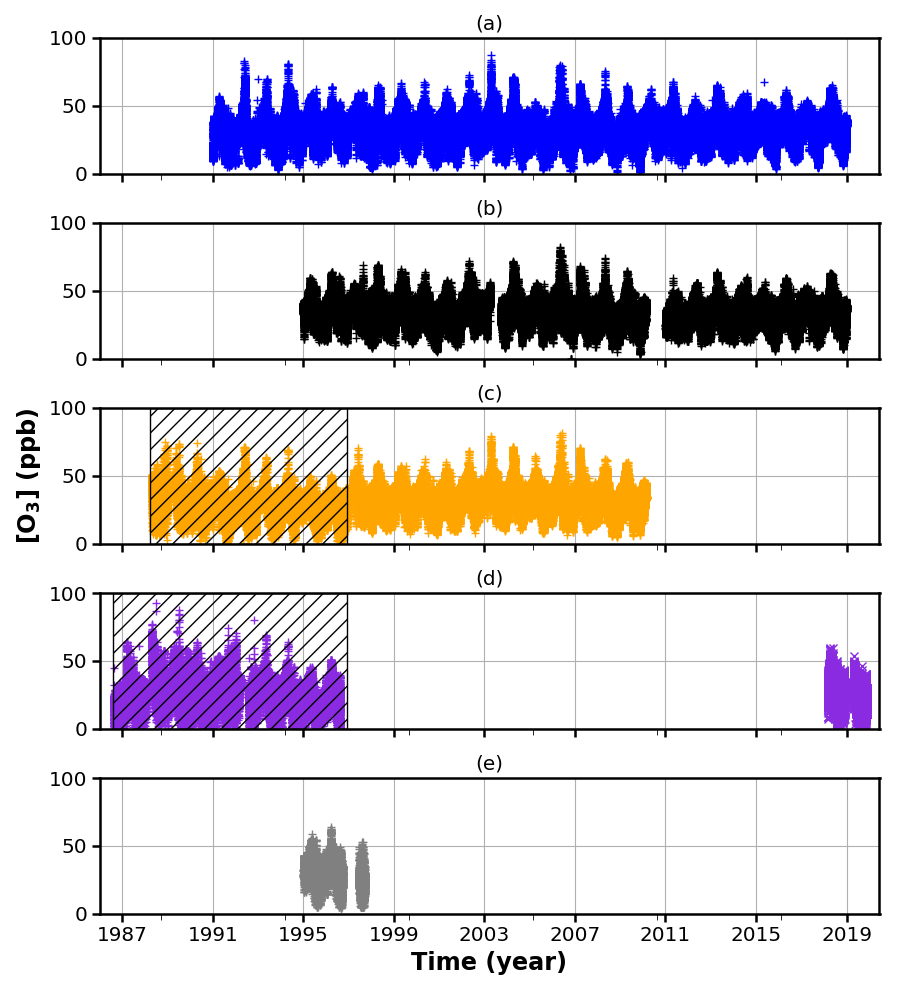
\includegraphics[width=12cm]{ozone_timeseries_fennoscandic_obs.png}
  \caption{Time series of ozone observations in northern Fennoscandia (Tab.~\ref{tab:ebas_obs}) (1986--2019). Data from EBAS until December 2018. The hatched areas indicate periods with insufficient quality control according to \citet{NILU2003}. (a) Esrange (SWE); (b) Janiskoski (RUS); (c) Jergul/Karasjok (NOR); (d) Pallas (FIN); (e) Svanvik (NOR).}
  \label{fig:ozone_timesseries_fenoscandic_obs}
\end{figure*}

%\begin{figure*}[t]
%  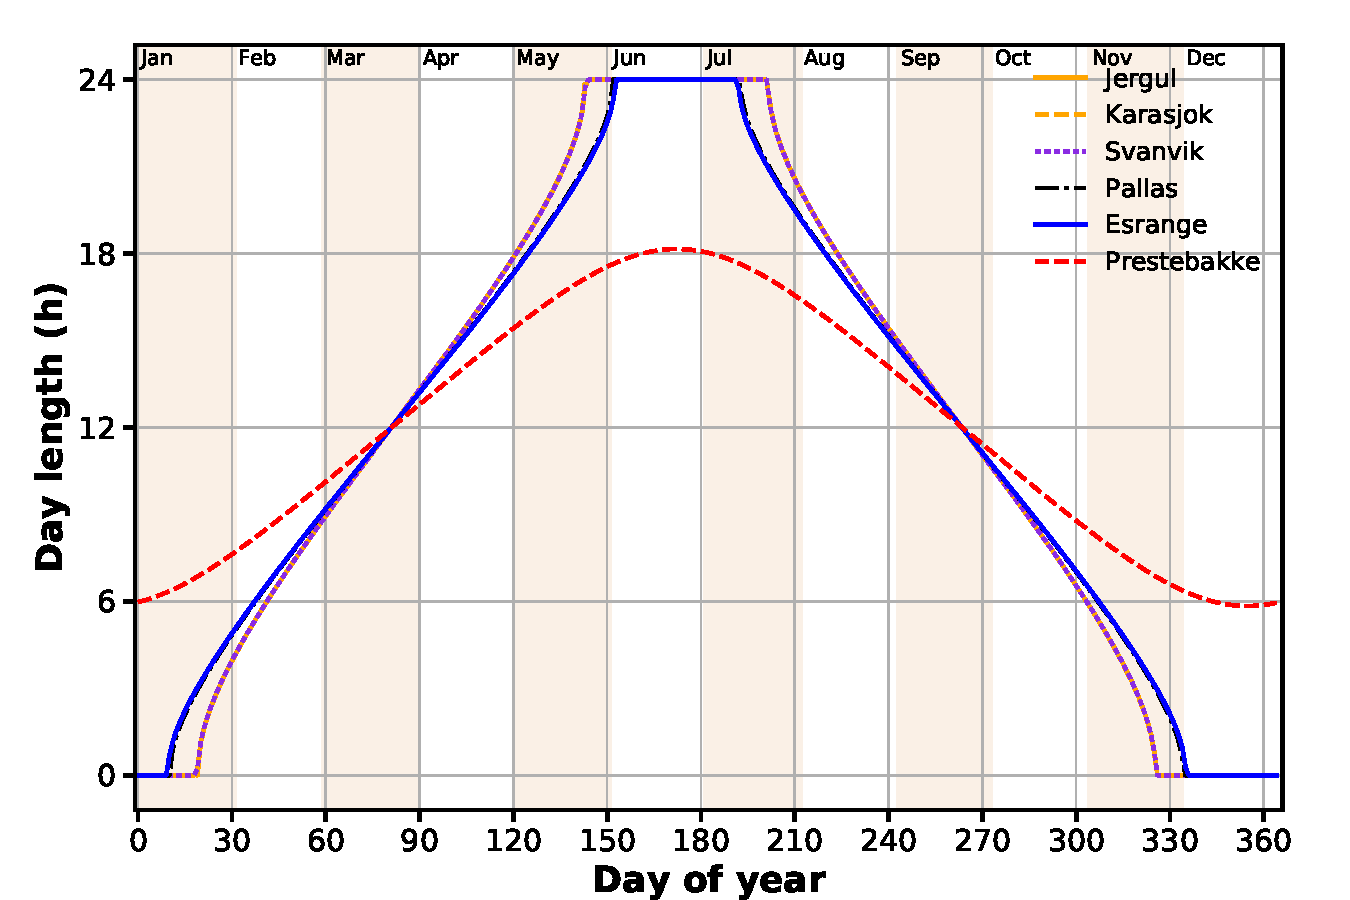
\includegraphics[width=12cm]{test_fennoscandia}
%  \caption{Maximum daily sun shine duration based on geometrical calculations at different sites in Fennoscandia. Midnight sun conditions at Jergul/Karasjok and Svanvik prevail from the end of May until the end of July, while at Esrange and Pallas they only prevail from the beginning of June until mid of July.}
%  \label{fig:sunlight_fennoscandia}
%\end{figure*}

%\begin{figure*}[t]
%  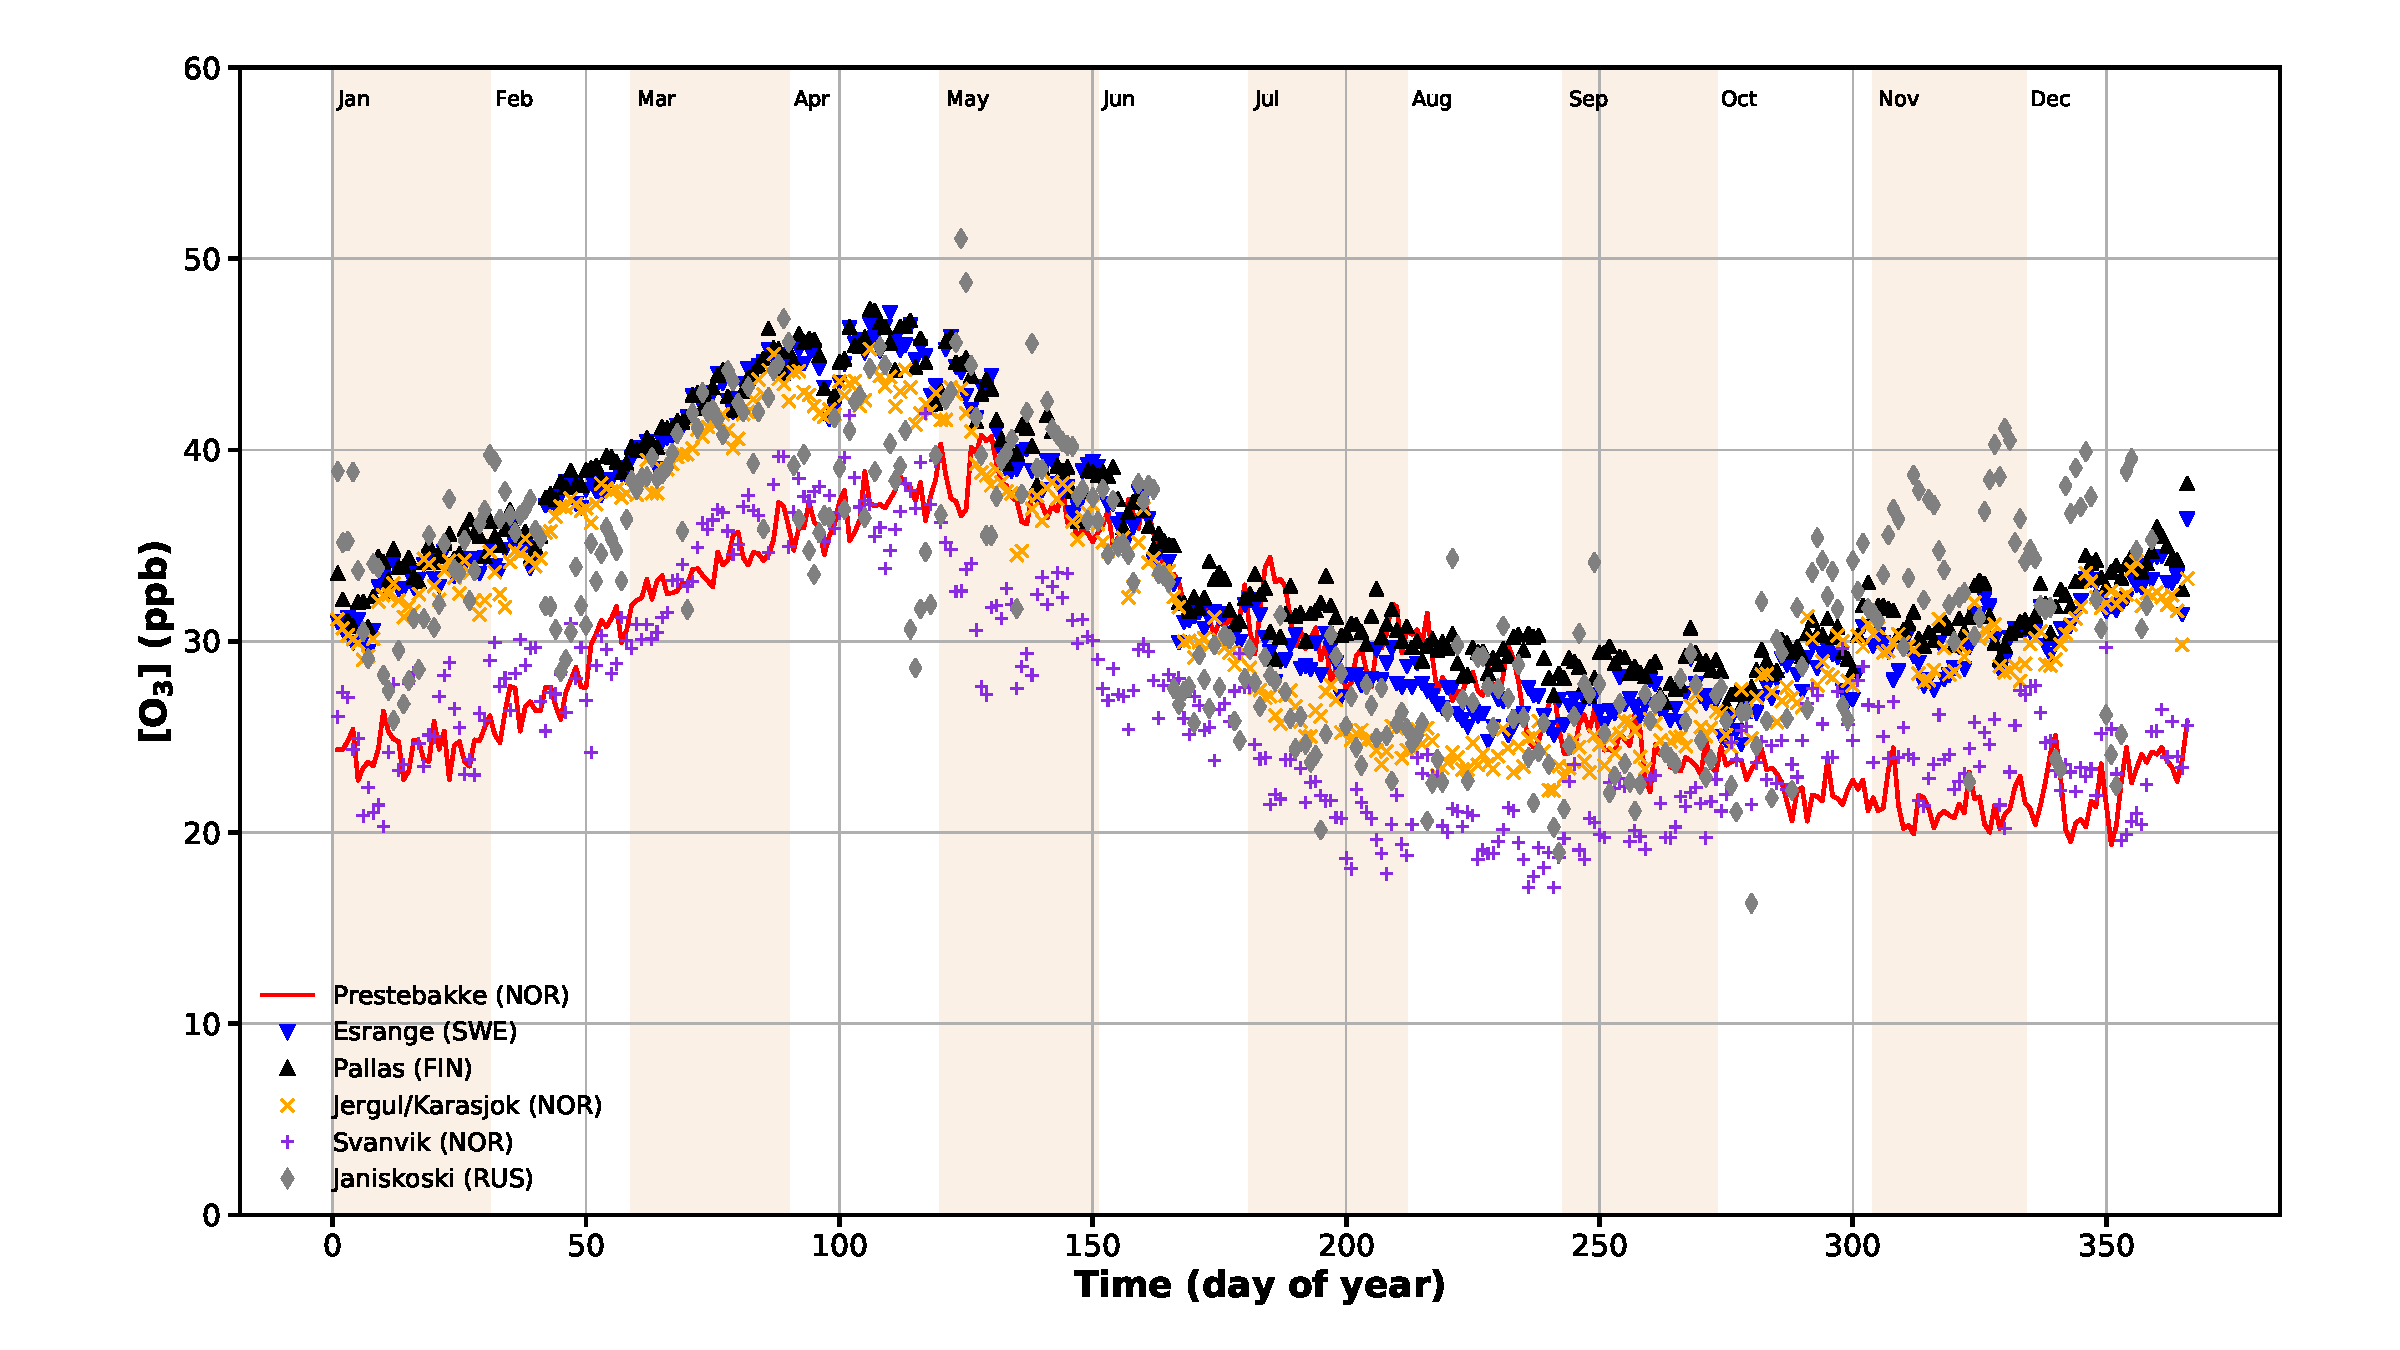
\includegraphics[width=12cm]{ozone_climatology_fenoscandic_obs}
%  \caption{Multi-annual mean of daily mean ozone at observation sites in Fennoscandia. The large spread in case of Svanvik and Janiskoski is due to the lower statistics. All climatologies peak in spring, with peak values in April. The annual average ozone concentration \chem{\left<[O_3]\right>} at Svanvik is $6.6\,\unit{ppb}$ lower than at the sites at Jergul/Karasjok (NOR), Esrange (SWE), and Pallas (FIN).}
%  \label{fig:ozone_climatology_fenoscandic_obs}
%\end{figure*}


\begin{figure*}[t]
  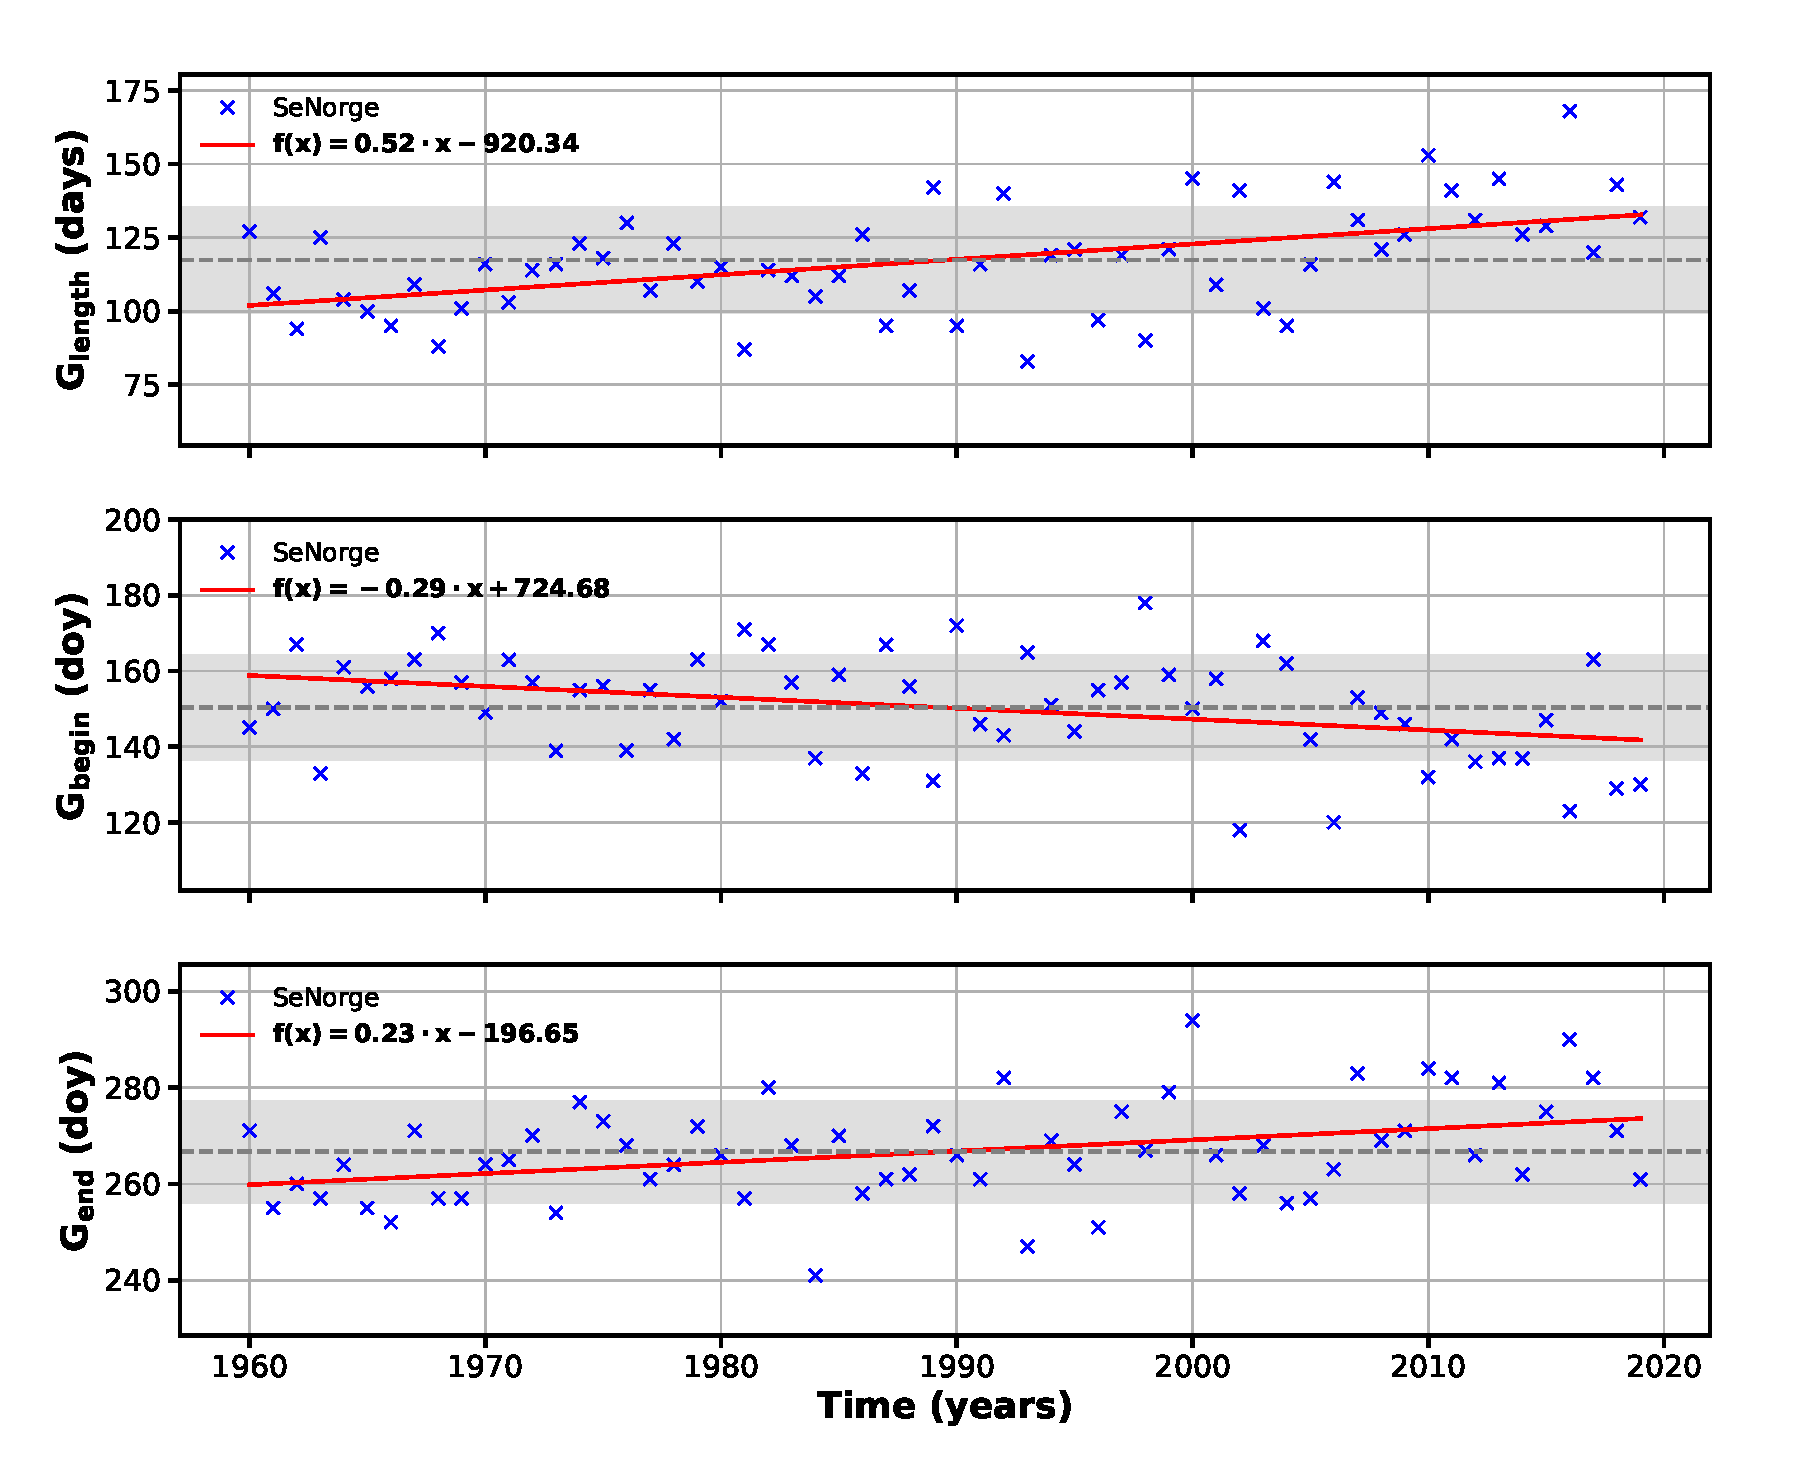
\includegraphics[width=12cm]{greening_season_change_Svanvik}
  \caption{Estimated shift and prolongation of greening season at Svanhovd over the past 6 decades based on data from \citet{SeNorge}.}
  \label{fig:greening_season_change_Svanvik}
\end{figure*}

\begin{figure*}[t]
  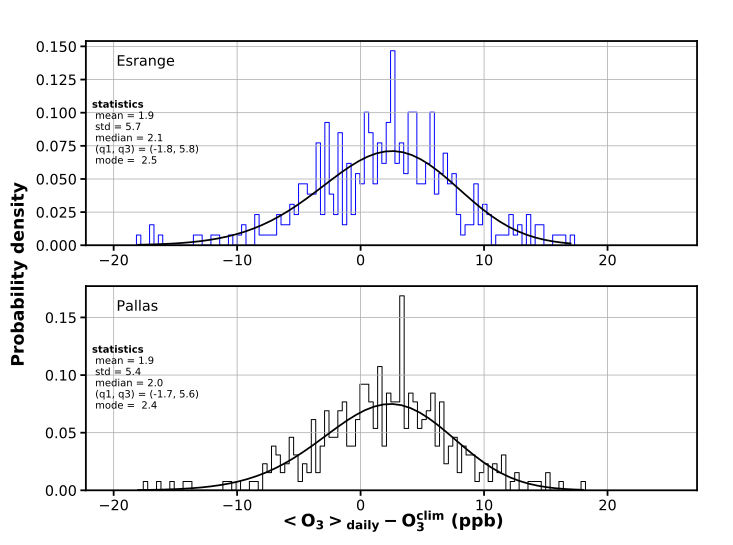
\includegraphics[width=12cm]{ozone_climatology_fenoscandic_obs_residuals}
  \caption{Probability density functions of ozone concentration residuals. 2018 with respect to respective climatology for different sites in Fennoscandia. (a) Esrange; (b) Pallas.}
  \label{fig:ozone_climatology_fenoscandic_obs_residuals}
\end{figure*}

\begin{figure*}[t]
  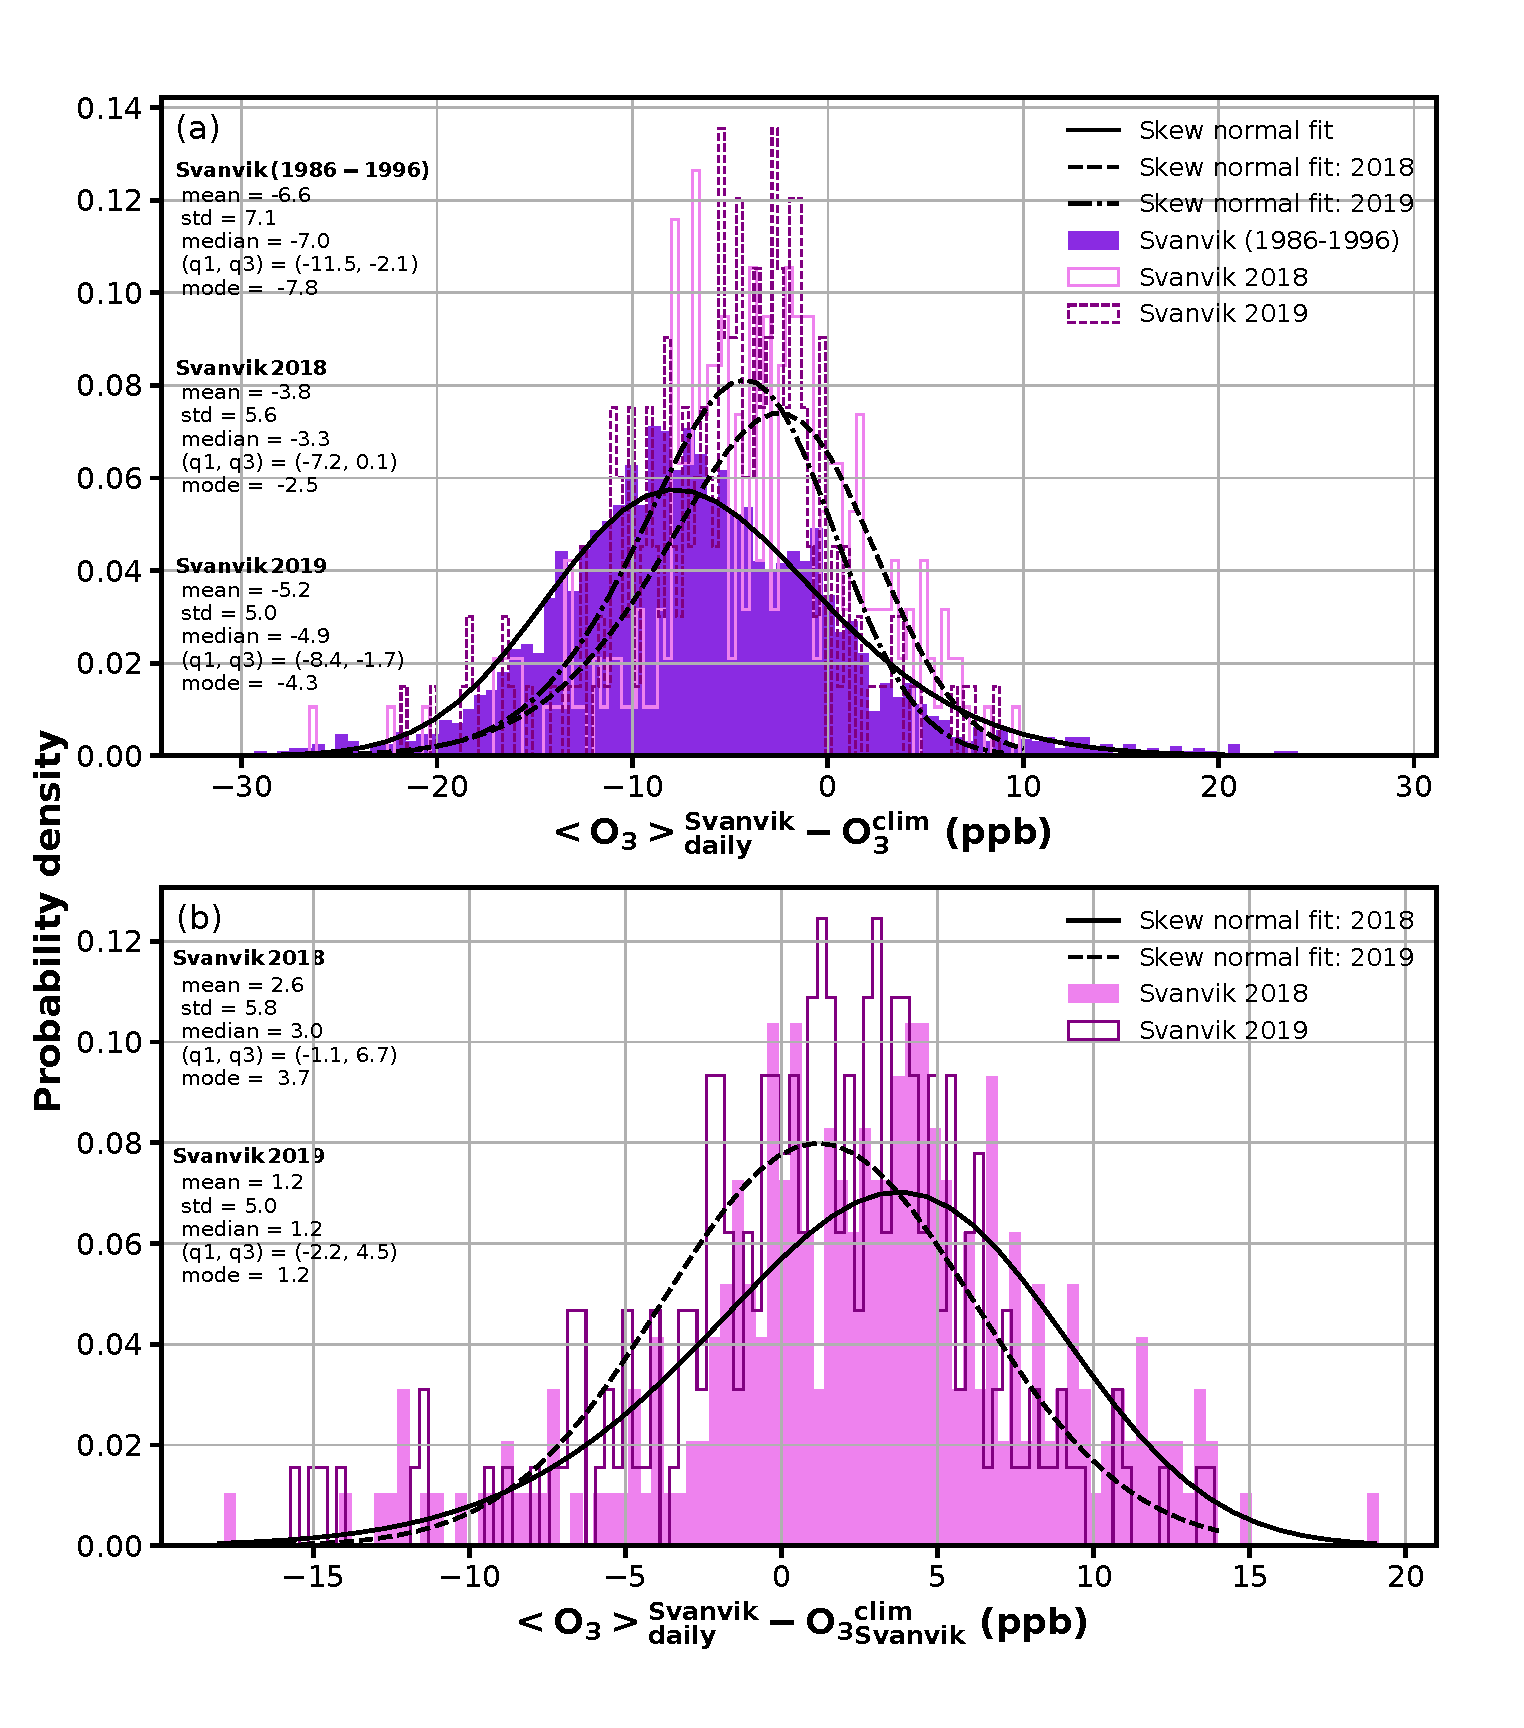
\includegraphics[width=12cm]{ozone_climatology_fenoscandic_obs_residuals-Svanvik}
  \caption{Probability density functions of ozone concentration residuals. 2018/19 observations at Svanhovd with respect to derived climatologies for (a) Northern Fennoscandia; (b) Svanvik.}
  \label{fig:ozone_climatology_fenoscandic_obs_residuals-Svanvik}
\end{figure*}

\begin{figure*}[t]
  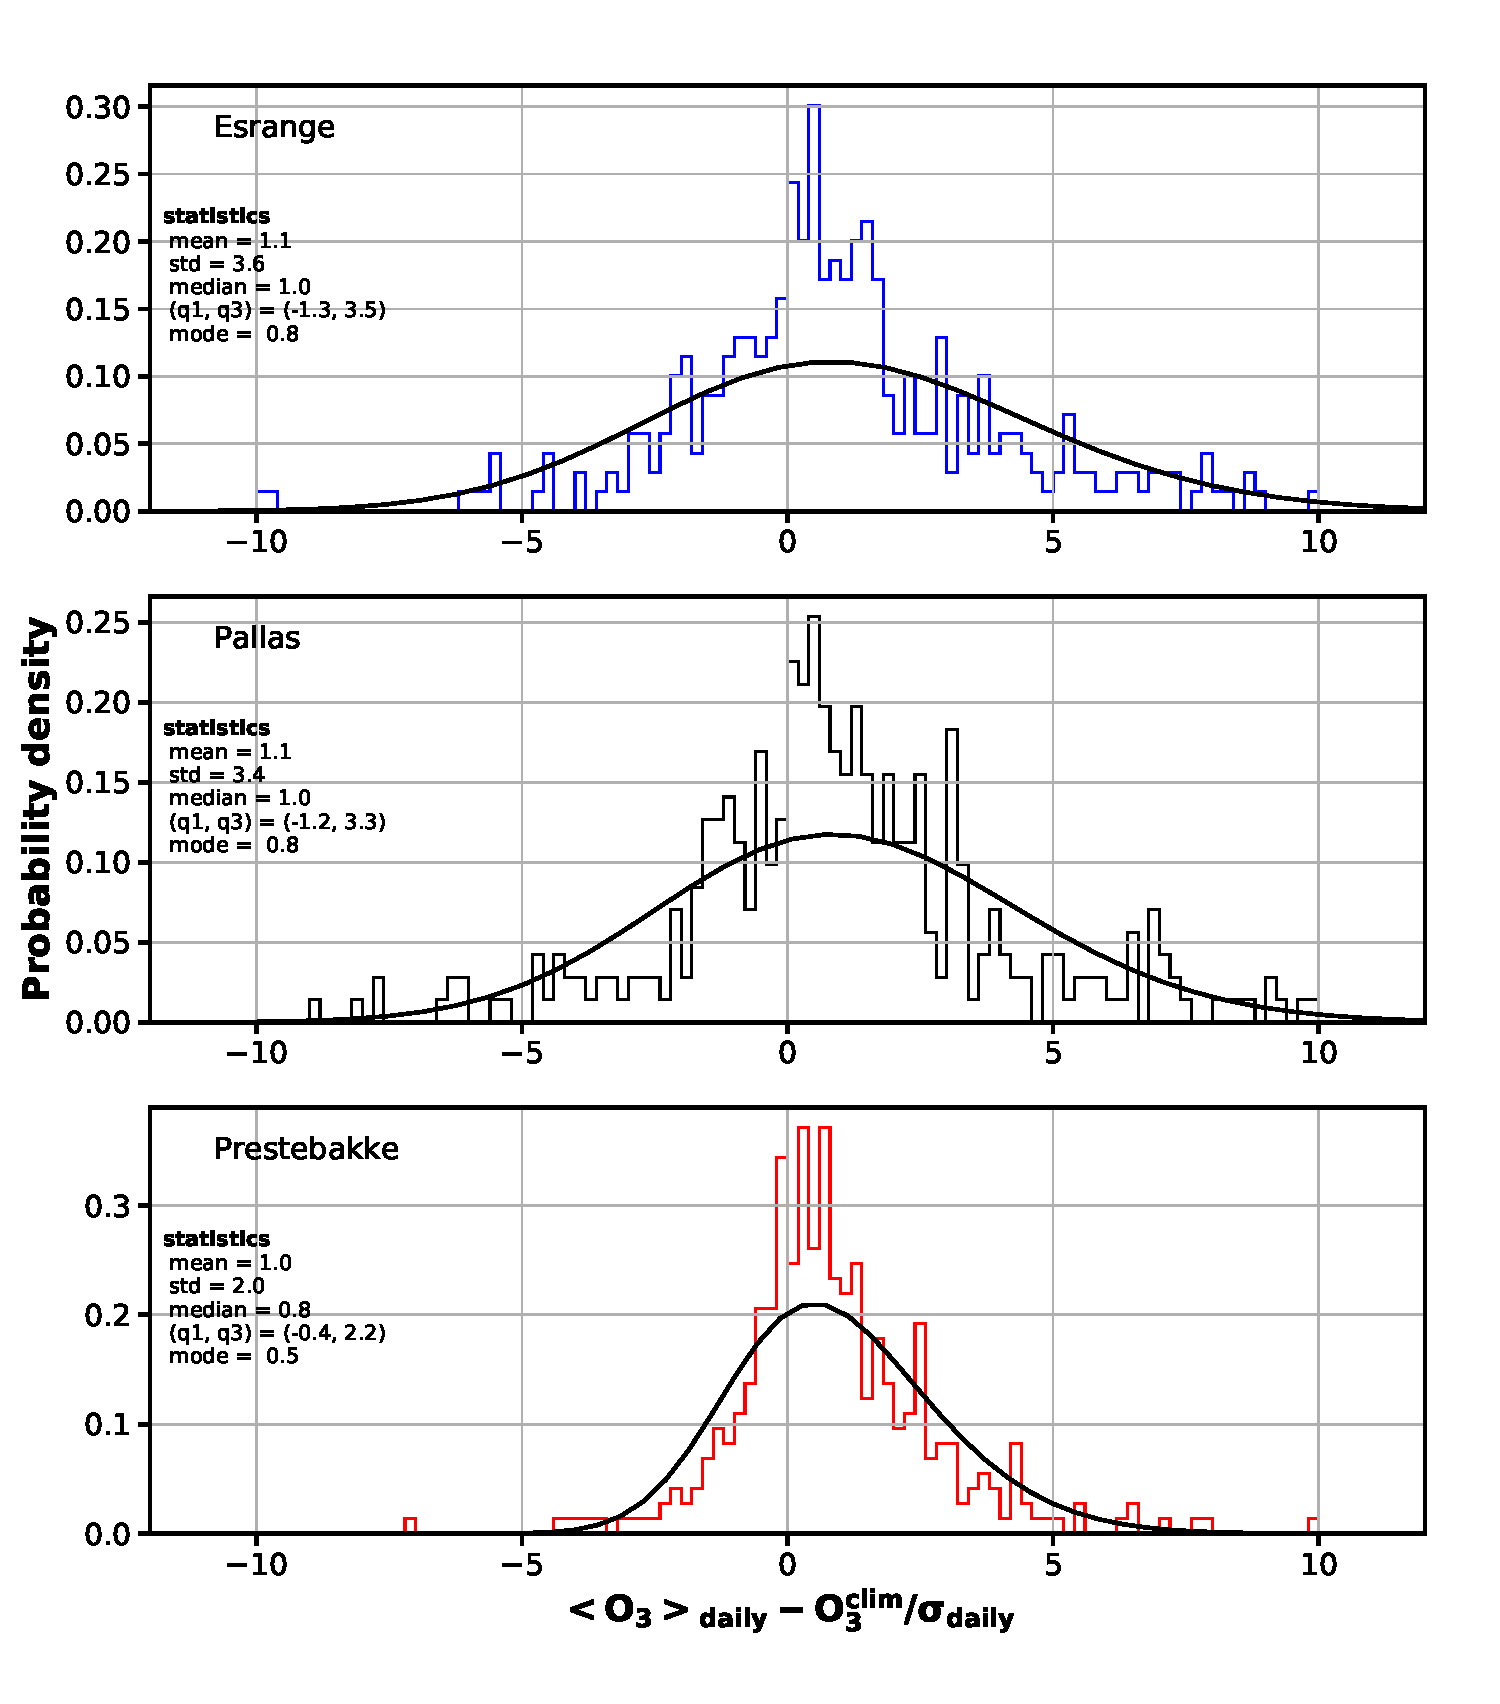
\includegraphics[width=12cm]{ozone_climatology_fenoscandic_obs_test}
  \caption{Student's t-test assuming same sample uncertainty in both, climatology and 2018 observations for different sites in Fennoscandia. \chem{\Delta[O_3]} in Fig.~\ref{fig:ozone_climatology_fenoscandic_obs_residuals} are significantly different from zero-hypothesis on the $1\,\sigma$ level. (a) Esrange; (b) Pallas.}
  \label{fig:ozone_climatology_fenoscandic_obs_test}
\end{figure*}

\begin{figure*}[t]
  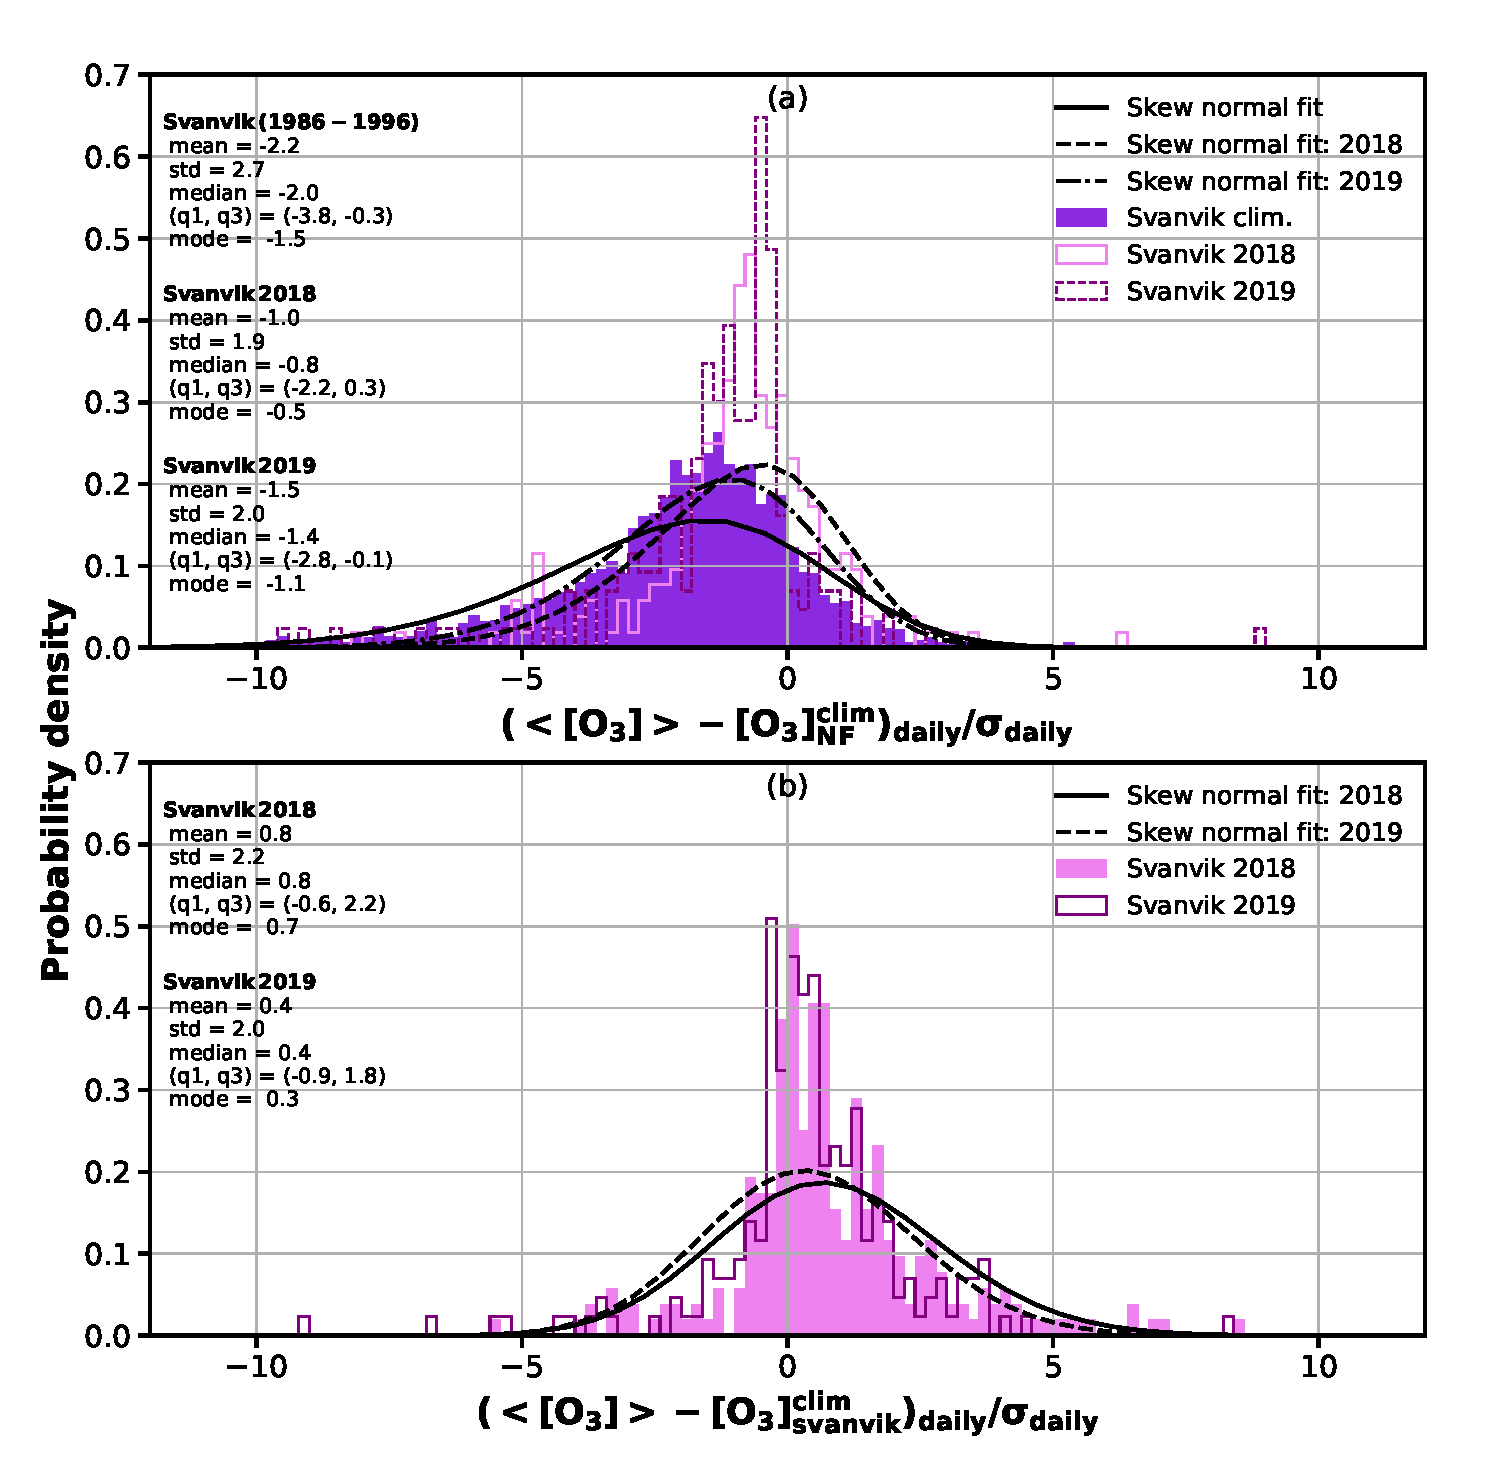
\includegraphics[width=12cm]{ozone_climatology_fenoscandic_obs_test-Svanvik}
  \caption{Student's t-test assuming same sample uncertainty in both, climatology and 2018/19 observations at Svanhovd with respect to derived climatologies for (a) Northern Fennoscandia; (b) Svanvik. \chem{\Delta[O_3]} in Fig.~\ref{fig:ozone_climatology_fenoscandic_obs_residuals}a) are significantly different from zero-hypothesis on the $2\,\sigma$,  $1\,\sigma$ level, respectively. \chem{\Delta[O_3]} in Fig.~\ref{fig:ozone_climatology_fenoscandic_obs_residuals}b) are not significantly different from zero-hypothesis.}
  \label{fig:ozone_climatology_fenoscandic_obs_test-Svanvik}
\end{figure*}

\begin{figure*}[t]
  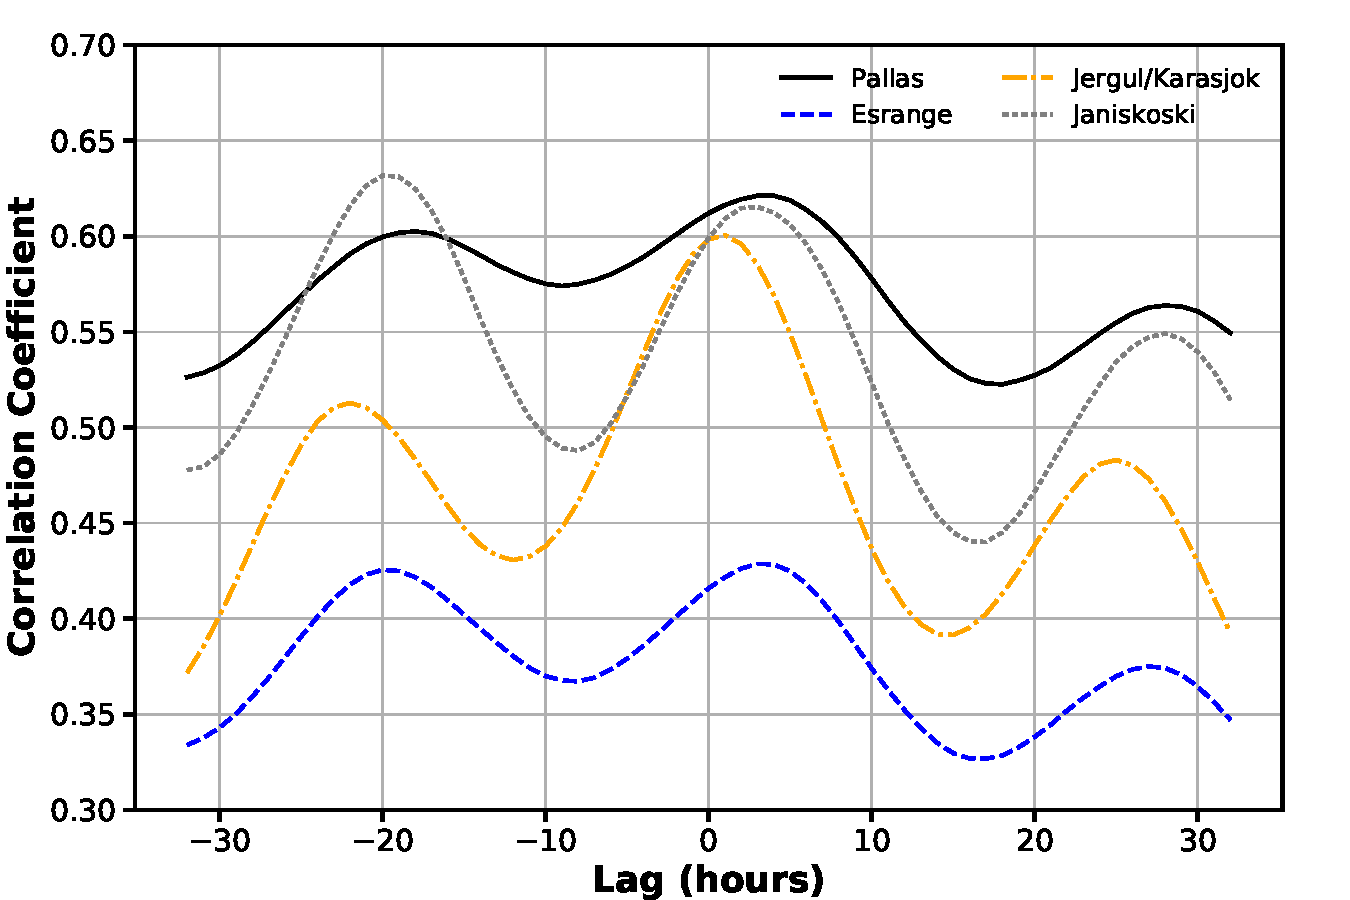
\includegraphics[width=12cm]{ozone_observation_timelag_svanvik}
  \caption{Temporal correlation of \chem{[O_3]} data at Svanvik with other ozone monitoring stations in northern Fennoscandia. A negative lag means that Svanvik lags behind, while a positive lag mean the other station lags behind. The highest correlation with Pallas/Esrange is found at a time lag of $3\,\unit{h}$, for Jergul/Karasjok at $1\,\unit{h}$, and for Janiskoski at $-20\,\unit{h}$.}
  \label{fig:time_lag_correlation}
\end{figure*}

%\begin{figure*}[t]
%  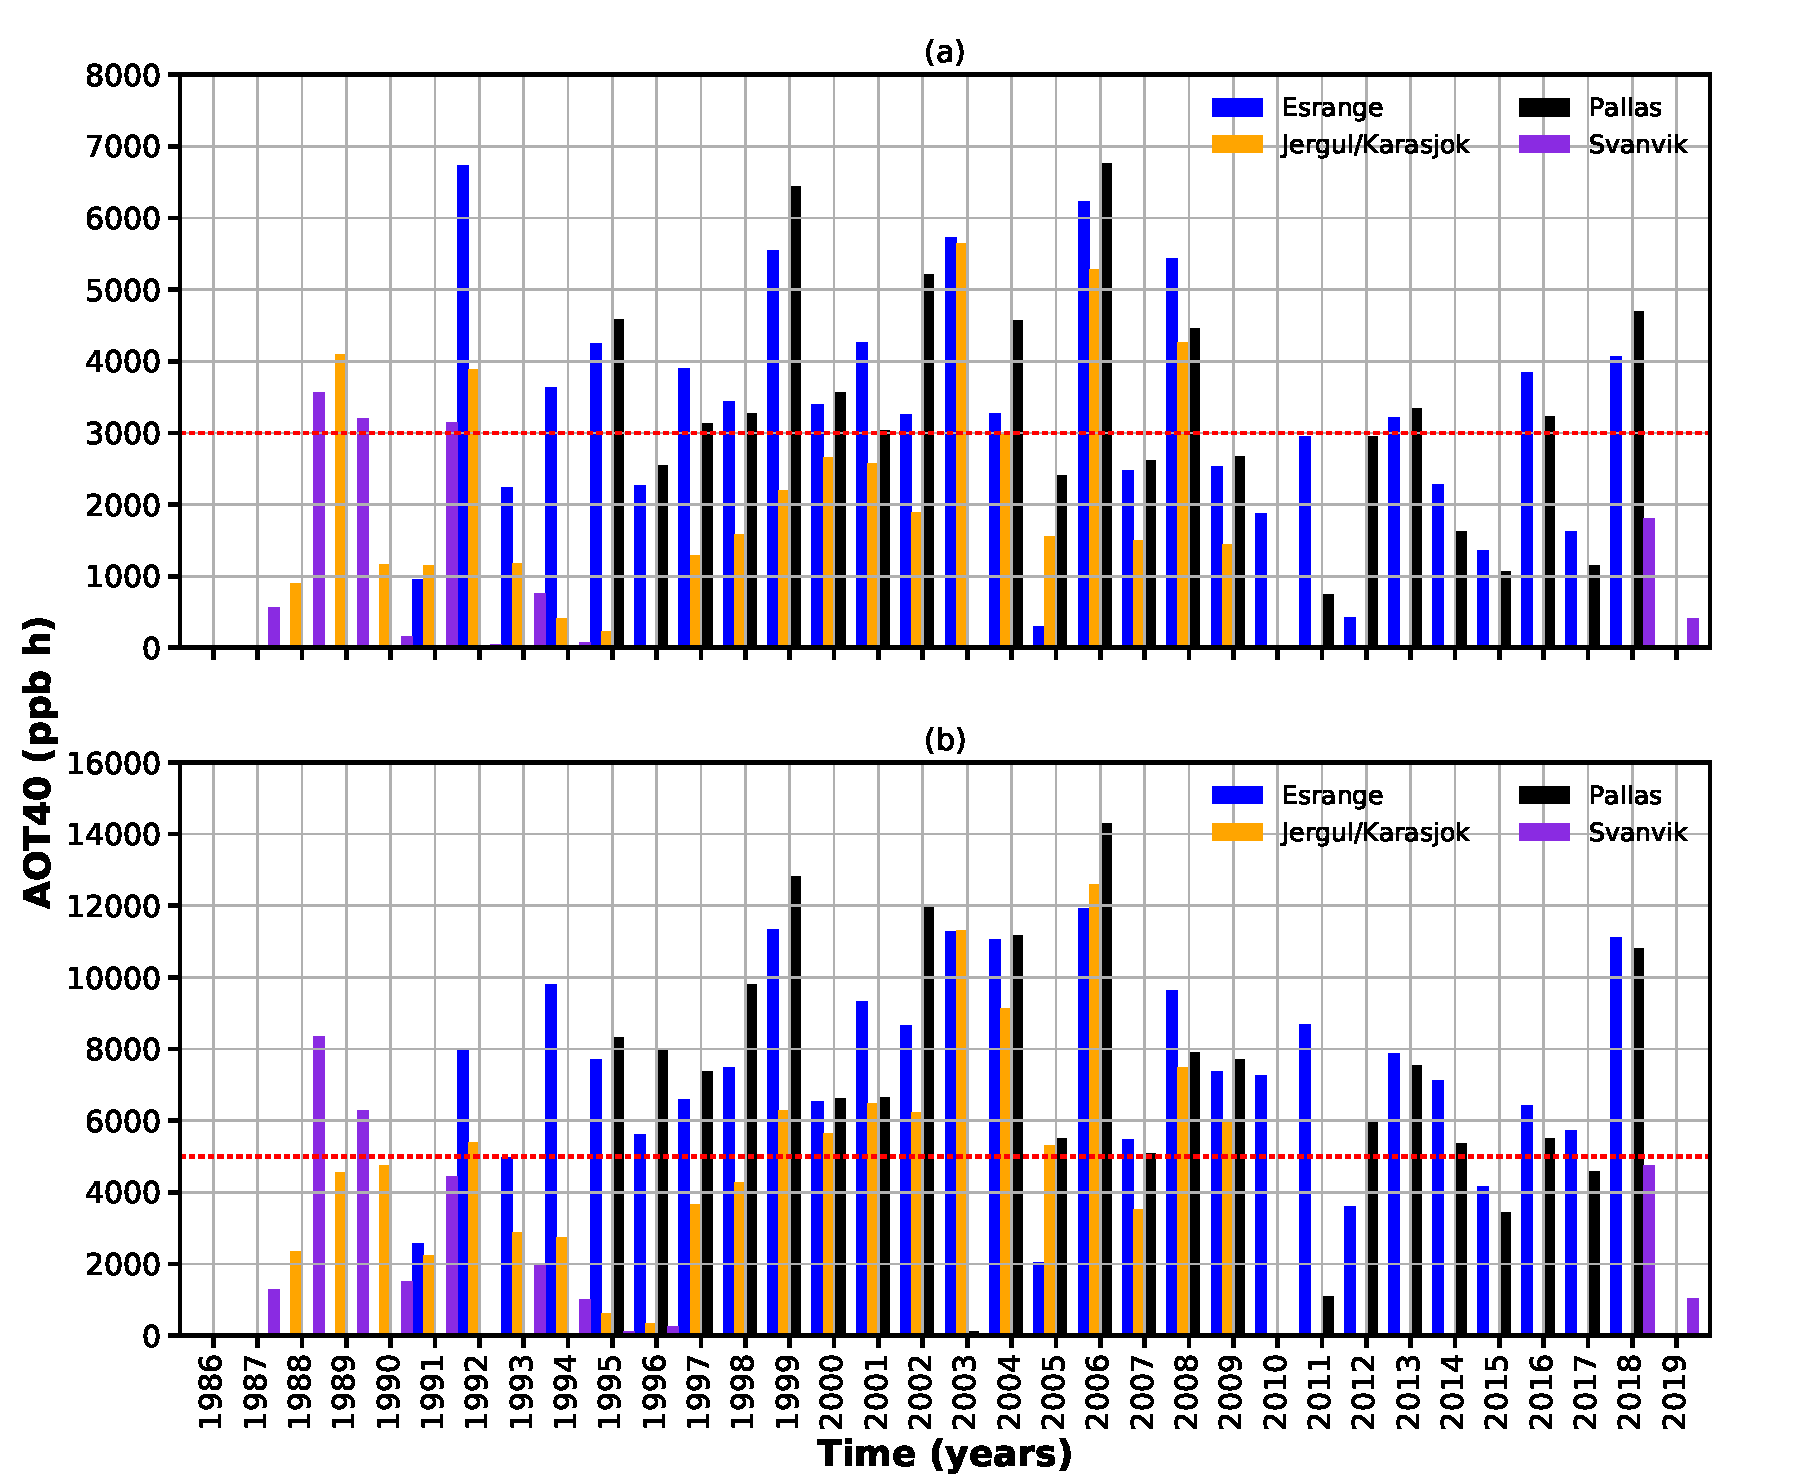
\includegraphics[width=12cm]{ozone_fennoscandic_obs_aot40}
%  \caption{Integrated AOT40 for various sites in northern Fennoscandia over the course of 33 years. For simplicity, we integrated hourly ozone between $1\,\unit{am}-11\,\unit{pm}$ in any case, although a night time light intensity $> 50\,\unit{W\,m^{-2}}$ is only measured during midnight sun conditions. Since night time \chem{[O_3]} is mostly below $40\,\unit{ppb}$, the such induced high bias in spring should be tolerable. The dashed red lines indicate the respective threshold given by the EU directive. (a) May 1 -- July 31 (b) April 1 -- September 30.}
%  \label{fig:fennoscandic_aot40}
%\end{figure*}

\begin{figure*}[t]
  \centering
  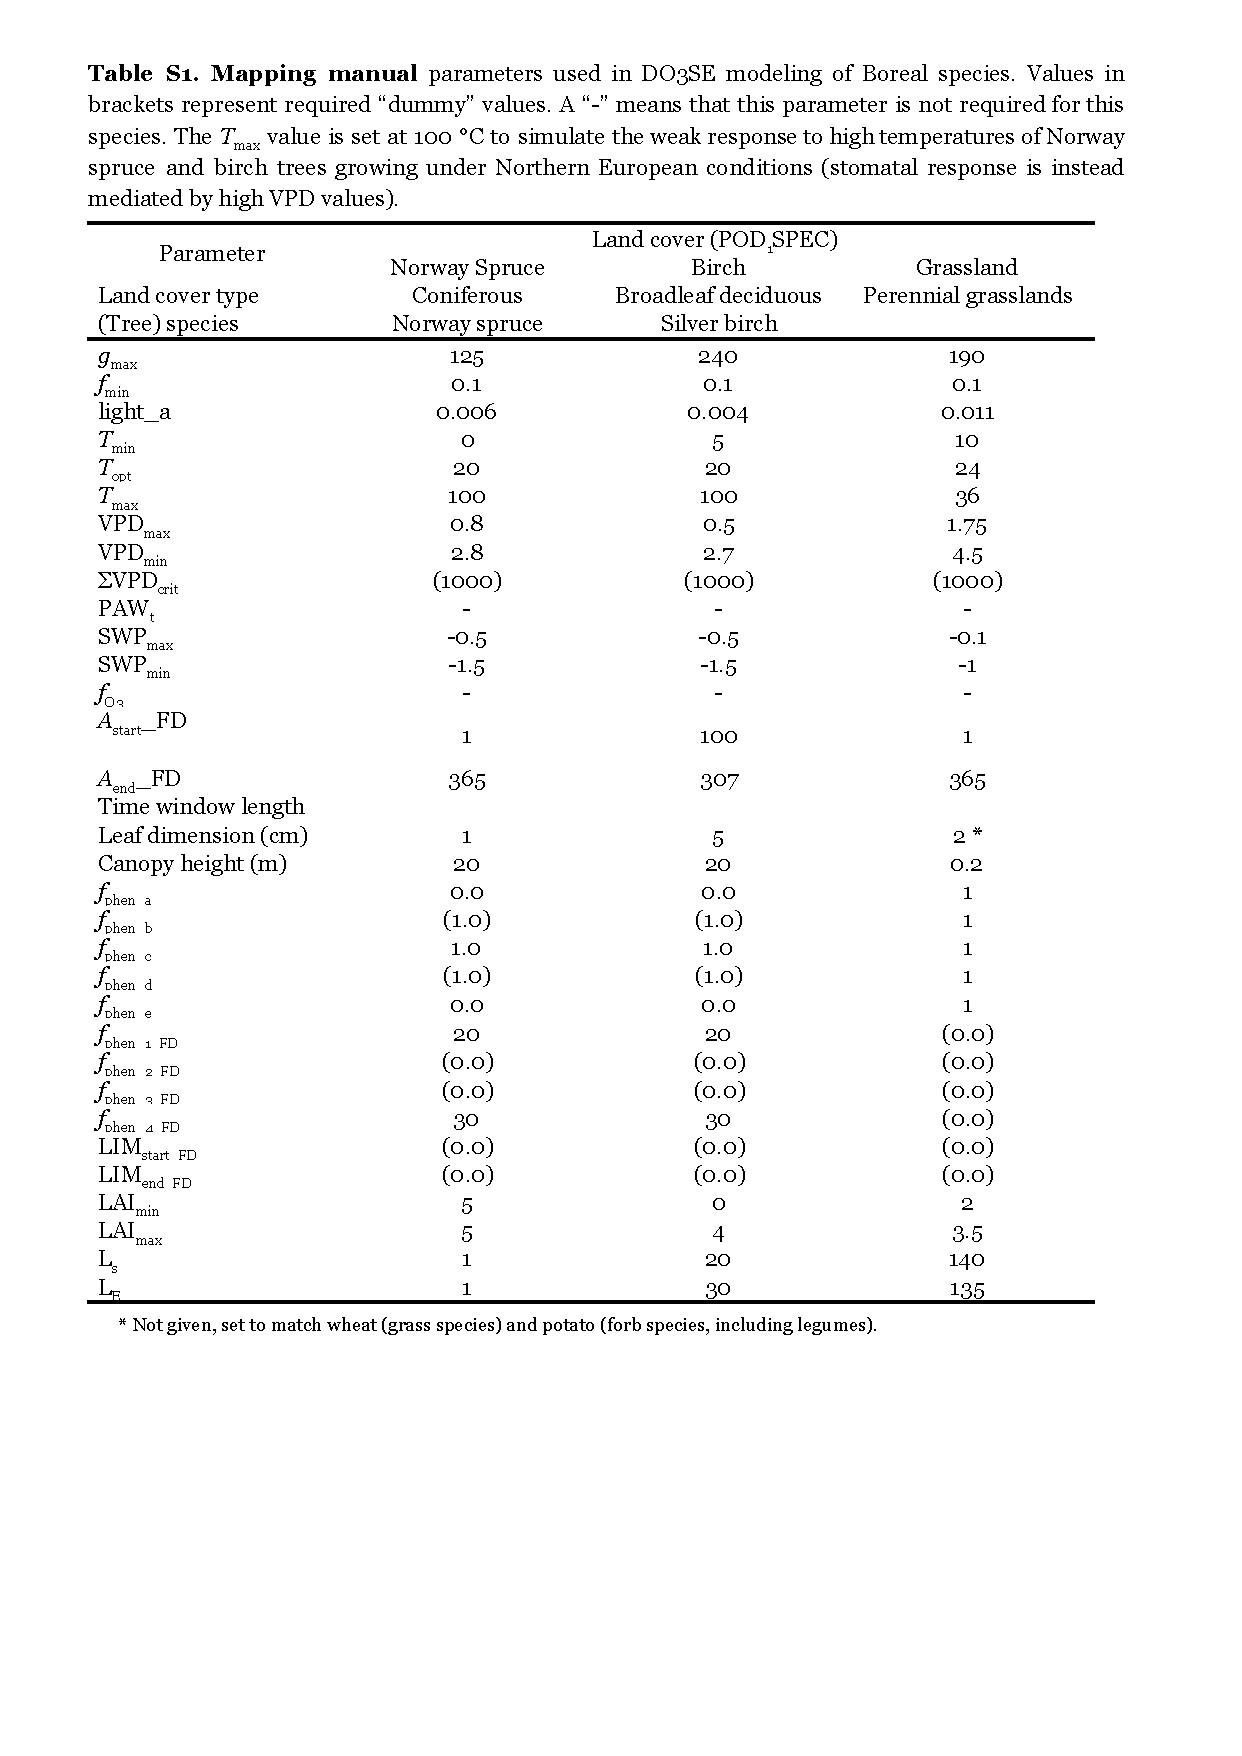
\includegraphics[width=1\textwidth]{supplements/supplement_do3se-parameterization_v2}
\label{tab:do3se_mm_param}
\end{figure*}
